\begin{figure}[hb!]
\resizebox{0.8\columnwidth}{!}{%
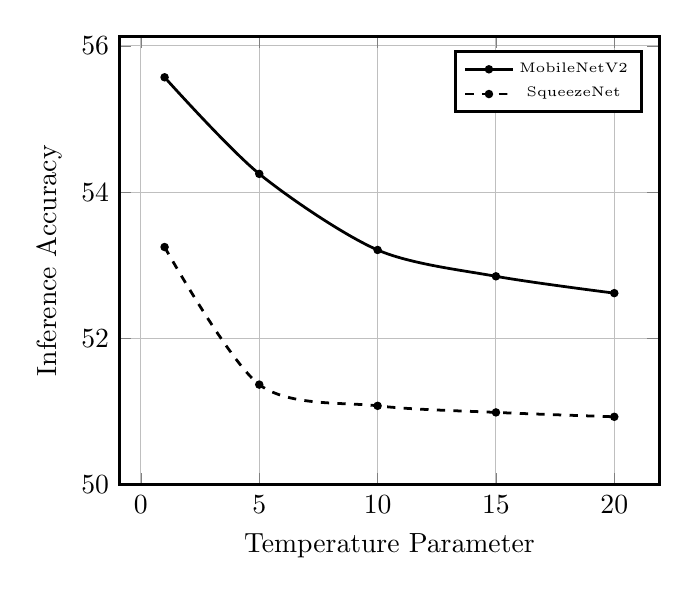
\begin{tikzpicture}
\begin{axis}[
legend style={font=\tiny},
legend pos =  north east,
line width=1.0pt,
mark size=1.0pt,
ymin=50,
legend entries={MobileNetV2, SqueezeNet},
ylabel={Inference Accuracy},
xlabel={Temperature Parameter},
% extra x ticks={1,10,...,400},
% extra y ticks={0,0.5,...,10},
% extra y tick labels={},
% extra x tick labels={},
% extra x tick style={grid=major},
% extra y tick style={grid=major},
grid=major
]
\addplot[
    color=black,
    solid,
    mark=*,
    mark options={solid},
    smooth
    ]
    coordinates {
    (1,55.57)(5,54.25)(10,53.21)(15,52.85)(20,52.62)
      };
\addplot[
      color=black,
      dashed,
      mark=*,
      mark options={solid},
      smooth
    ]
    coordinates {
    (1,53.25)(5,51.37)(10,51.08)(15,50.99)(20,50.93)
      };
\end{axis}
\end{tikzpicture}
}
\caption{The privacy leakage of models designed for efficiency (SqueezeNet and MobileNet) can be reduced by increasing the softmax temperature. }
\end{figure}
